% Live Layer Protocol: research paper.
% Build: cd paper && make   (pdflatex + bibtex; see paper/README.md)
\documentclass[10pt,twocolumn]{article}
\usepackage[T1]{fontenc}
\usepackage[utf8]{inputenc}
\usepackage{lmodern}
\usepackage[margin=0.85in,columnsep=0.3in]{geometry}
\usepackage{microtype}
\usepackage{booktabs}
\usepackage{array}
\usepackage{tabularx}
\usepackage{graphicx}
\usepackage{xcolor}
\usepackage{listings}
\usepackage{tikz}
\usetikzlibrary{arrows.meta,positioning,calc}
\usepackage{pgfplots}
\pgfplotsset{compat=1.18}
\usepackage[hyphens]{url}
\usepackage[colorlinks=true,linkcolor=black,citecolor=black,urlcolor=black]{hyperref}
\usepackage{enumitem}
\setlist{nosep,leftmargin=1.3em}

% Author line: change here.
\newcommand{\paperauthor}{Nikhil Ajay Kadalge}
\newcommand{\paperaffil}{Independent}
\newcommand{\repo}{\url{https://github.com/nik190799/live-layer-protocol}}
\newcommand{\paperemail}{\href{mailto:nikhil.kadalge@gmail.com}{nikhil.kadalge@gmail.com}}
\newcommand{\paperorcid}{ORCID: \href{https://orcid.org/0009-0004-8859-5607}{0009-0004-8859-5607}}

\lstset{basicstyle=\ttfamily\footnotesize,breaklines=true,columns=fullflexible,
  frame=single,framerule=0.3pt,rulecolor=\color{black!40},xleftmargin=2pt,xrightmargin=2pt,
  aboveskip=6pt,belowskip=4pt,showstringspaces=false}
\newcommand{\code}[1]{\texttt{#1}}
\usepackage{xspace}
\newcommand{\ms}{\,ms\xspace}
\newcommand{\s}{\,s\xspace}
\renewcommand{\arraystretch}{1.08}
\sloppy

\title{\textbf{Live Layer Protocol: Streaming Signed, Verified WebAssembly Layers into Running Applications}}
\author{\paperauthor\\{\small \paperaffil}\\{\small\paperemail \quad \paperorcid}\\{\small\repo}}
\date{November 2026 \quad (v0 preprint)}

\begin{document}
\maketitle

\begin{abstract}
Shipping a code change today means running it through a build--test--release--deploy pipeline and
then restarting the program that runs it. The pipeline is where safety checks live, so it cannot
simply be removed. We describe the Live Layer Protocol (LLP), which moves those checks to the moment
a change arrives at a running application. Code is delivered as a stream of small, signed,
content-addressed WebAssembly modules (\emph{layers}). A \emph{Live Host} owns all application
state, verifies each signed manifest, rehearses the new layers against a copy-on-write shadow of
the real state, commits all of them atomically or none, and reverts a layer that traps or exceeds
its time or memory limit. The same manifest stream drives client devices and server or edge nodes,
and a fleet layer adds channels, percentage rollouts with health gates, convergence tracking and
key rotation. We report a reference host in JavaScript, an independent second host in Go written
from the specification, and a conformance suite of 161 language-neutral checks that both pass.
On one 4-core machine, a warm swap takes 2.3\ms (p50), a change reaches 1{,}000 simulated hosts
0.58\s after the file is saved, and a layer that crashes after going live is reverted with state
restored in 2.3\ms. A red-team review produced 39 findings, of which 29 are fixed (several only
partly or opt-in) and 10 remain open. We replay the failure mechanisms of four public outages in
simulation and state where the protocol contains the failure and where it does not. LLP v0 is
experimental: it catches crashes and hangs, not wrong answers, and several results come from
single-machine simulation.
\end{abstract}

\section{Introduction}

A running program and the code a developer just wrote are separated by a pipeline. The change is
committed, built, tested, packaged, pushed to a registry, rolled out, and the process that serves
users is restarted on the new build. Continuous delivery~\cite{humble2010cd} made this pipeline
fast and repeatable, but it did not make it disappear. Industry reports put the average CI workflow
at 2\,min\,49\s~\cite{circleci2024} and the lead time of the best-performing teams at under one
day~\cite{dora2024}. The restart at the end discards in-memory state and, for a client application,
often the user's unsaved work.

The pipeline exists for good reasons. It is where a change is checked before users meet it. A
proposal to remove it must say where those checks go. The need is sharper now that language
models write a growing share of changes: code can be produced in seconds, so the minutes between
``written'' and ``running'' are a larger share of the loop, and the code was not read line by line by
the person who asked for it.

This paper describes the \emph{Live Layer Protocol} (LLP). Its position is that verification
should happen \emph{at the moment a change arrives at the running program}, against that
program's real state, and that the unit of delivery should be small enough to verify and swap in
milliseconds. Concretely:

\begin{itemize}
\item Code ships as \textbf{layers}: WebAssembly modules~\cite{haas2017wasm}, from any source
language, identified by the SHA-256 of their bytes.
\item A \textbf{signed, monotonic manifest} names the layers of one release. Hosts accept only
manifests signed by a trusted key, for their own application, with a higher version.
\item \textbf{State lives in the host}, never in a layer, so replacing code cannot lose it.
\item A new layer is \textbf{rehearsed on a shadow copy} of the real state (load, migrate, render)
and committed only if that succeeds. A multi-layer manifest commits entirely or not at all.
\item Each layer call is a \textbf{transaction} with a time and memory budget. A trap or a
breach discards the call's writes and reverts the layer to its previous version.
\end{itemize}

\paragraph{Contributions.}
\begin{enumerate}
\item The design of LLP: manifest, wire messages, swap algorithm, layer ABI and sandbox limits
(\S\ref{sec:design}); its extension to server and edge hosts and to fleets with staged rollouts
and TUF-style key rotation (\S\ref{sec:beyond}); and a publishing loop in which a language model
writes the layer (\S\ref{sec:ai}).
\item Two independent implementations, in JavaScript and Go, and a conformance suite of 161
checks, with the 16 specification defects that writing the second implementation exposed
(\S\ref{sec:impl}).
\item A measured evaluation of swap cost, fleet convergence, rollback and a rebuild-and-restart
baseline on the same machine (\S\ref{sec:eval}), including where the conventional path is
\emph{not} slow.
\item A simulated replay of the failure mechanisms of four public outages, with the cases LLP
does not help stated alongside those it does (\S\ref{sec:cases}).
\item A red-team review with a threat model and the status of every finding, including those
still open (\S\ref{sec:security}).
\end{enumerate}

\paragraph{Scope and honesty.} LLP is at version 0. Every number in this paper was produced by a
script in the public repository and re-run for this paper on one cloud VM
(\S\ref{sec:setup}). Fleets are simulated on that machine. The outage replays reproduce a failure
\emph{mechanism} in a few dozen lines; they are not claims that LLP would have prevented the real
incidents. No production deployment exists yet.

\section{Background and Motivation}
\label{sec:background}

\paragraph{What the pipeline costs.} The DORA 2024 report places elite teams at on-demand deploys
with a lead time under one day, a 5\% change failure rate and recovery in under an
hour~\cite{dora2024}; fewer than 20\% of surveyed organisations are in that cluster. CircleCI's
2024 data reports an average workflow of 2\,min\,49\s and an average recovery time of
57\,min~\cite{circleci2024}. These are cited figures, not measurements of ours. We note that an
earlier draft of this project assumed far worse numbers (10--40\,min CI); the published data did
not support them, and we corrected the claim.

\paragraph{What a restart costs.} A process restart is cheap on one machine (we measure 41\ms in
\S\ref{sec:baseline}). What it costs is state: anything held in memory is gone, connections drop,
and a client page reload discards unsaved input. Systems that avoid this, such as Erlang/OTP's
release handling~\cite{armstrong2003}, do so by separating long-lived state from replaceable code
and by giving the new code a hook to convert the old state.

\paragraph{What a bad change costs.} Several widely reported outages share one shape: a change
reached many machines before anything had checked that it worked on those
machines~\cite{crowdstrike2024rca,cloudflare2019,fastly2021,sec2013knight}. Staged rollout with
health gates is the standard remedy~\cite{li2020gandalf,tang2015config}, but it is a property of
the deployment system, and paths that bypass that system (content updates, rule pushes,
configuration) bypass the remedy too.

\paragraph{Design goal.} Deliver a change to a running application in milliseconds, without
losing state, on any operating system and from any source language, while keeping (and moving
closer to the user) the checks the pipeline provided: authenticity, integrity, a pre-flight run,
staged exposure and automatic rollback.

\section{Design}
\label{sec:design}

\subsection{Roles and principles}

A \textbf{layer} is a WebAssembly module implementing the LLP ABI; it holds no state. A
\textbf{Live Host} runs layers and owns state, permissions, rendering and the swap engine. A
\textbf{publisher} (a person or an AI agent) compiles layers, signs manifests and streams them. A
\textbf{layer store} is any source of content-addressed blobs.

The specification fixes nine principles: those in the introduction, and further that capabilities are
requested from the host and never assumed; the same layer runs on a client or a server host, with
placement a manifest field; layers never run on the host's thread; and a host with no trusted keys
refuses everything (fail closed).

\subsection{Manifest}

\begin{lstlisting}
{ "app": "demo.tasks", "version": 2,
  "layers": { "main": "<sha256>",
              "footer": "<sha256>" },
  "order": ["main", "footer"] }
\end{lstlisting}

A manifest maps named \emph{slots} to layer hashes. It is signed with ECDSA P-256/SHA-256 over
its canonical JSON form (RFC~8785~\cite{rfc8785}, restricted to I-JSON~\cite{rfc7493}); the
signature travels beside it as 64-byte $r\Vert s$. \code{version} is a positive safe integer and
an optional \code{epoch} orders releases ahead of it, so manifests compare as
$(\mathit{epoch},\mathit{version})$. A host accepts an epoch only up to the number of the keyring
it trusts (\S\ref{sec:keys}), which lets a key rotation outrank any version a leaked key signed.
A version more than one year of milliseconds ahead of the host's clock is refused, so a single
enormous version cannot freeze future updates. Optional signed fields place slots on hosts
(\code{hosts}), restrict the state keys (\code{keys}) and capabilities (\code{caps}) of each slot,
mark private and personal data prefixes, and carry the fleet fields \code{channel} and
\code{rollout}. A manifest declaring \code{"llp": 1} is strict: unknown fields are refused and
\code{keys} and \code{caps} are mandatory.

\subsection{Stream messages}

LLP is transport-agnostic JSON; the reference transports are WebSocket and, in browsers,
\code{BroadcastChannel}. Five messages suffice (Figure~\ref{fig:protocol}). A host announces the
hashes it already holds, so only changed layers are transferred. A refusal carries a
machine-readable \code{code} (\code{malformed}, \code{untrusted}, \code{wrong\_app},
\code{protocol}, \code{bad\_version}, \code{stale}, \code{blob}, \code{layer\_failed}) naming the
step that refused it.

\begin{figure}[t]
\centering
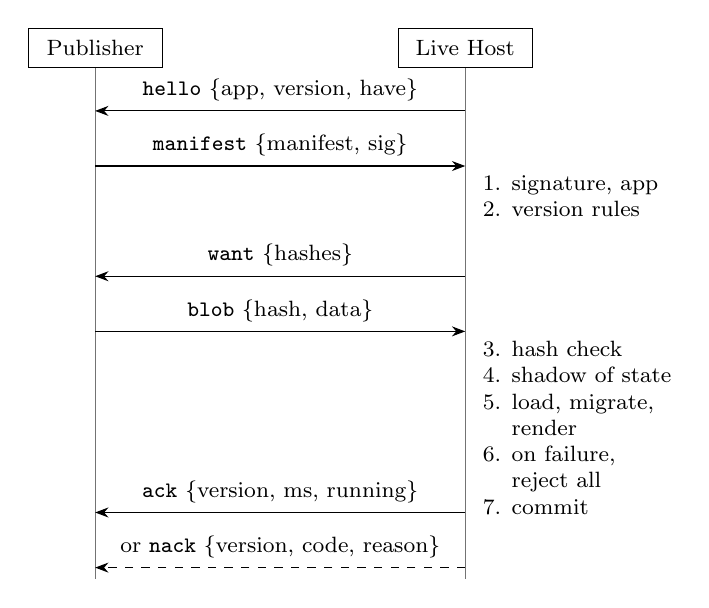
\begin{tikzpicture}[font=\footnotesize,>=Stealth,x=1cm,y=1cm]
  \node[draw,minimum width=1.7cm,minimum height=0.5cm] (P) at (0,0) {Publisher};
  \node[draw,minimum width=1.7cm,minimum height=0.5cm] (H) at (4.7,0) {Live Host};
  \draw[black!55] (P.south) -- (0,-6.75);
  \draw[black!55] (H.south) -- (4.7,-6.75);
  \draw[->] (4.7,-0.8) -- node[above]{\code{hello} \{app, version, have\}} (0,-0.8);
  \draw[->] (0,-1.5) -- node[above]{\code{manifest} \{manifest, sig\}} (4.7,-1.5);
  \node[anchor=north west,align=left] at (4.8,-1.5) {1. signature, app\\2. version rules};
  \draw[->] (4.7,-2.9) -- node[above]{\code{want} \{hashes\}} (0,-2.9);
  \draw[->] (0,-3.6) -- node[above]{\code{blob} \{hash, data\}} (4.7,-3.6);
  \node[anchor=north west,align=left] at (4.8,-3.6) {3. hash check\\4. shadow of state\\5. load, migrate,\\\phantom{5. }render\\6. on failure,\\\phantom{6. }reject all\\7. commit};
  \draw[->] (4.7,-5.9) -- node[above]{\code{ack} \{version, ms, running\}} (0,-5.9);
  \draw[->,dashed] (4.7,-6.6) -- node[above]{or \code{nack} \{version, code, reason\}} (0,-6.6);
\end{tikzpicture}
\caption{The LLP stream and the host's swap steps. The running version is untouched until step~7.}
\label{fig:protocol}
\end{figure}

\subsection{Swap algorithm}
\label{sec:swap}

On receiving a manifest the host:
\begin{enumerate}
\item rejects it if the host has no trusted keys or no pinned application, if no trusted key
made the signature, or if it names another application;
\item rejects it unless $(\mathit{epoch},\mathit{version})$ is in range and strictly greater than
the running pair (anti-rollback, anti-replay, anti-freeze);
\item fetches missing blobs and rejects any whose SHA-256 differs from the declared hash;
\item opens a copy-on-write shadow of state, whose cost is proportional to the keys written;
\item for each changed slot placed on this host, in sorted slot order: instantiates the layer,
calls \code{llp\_migrate(from)} if its schema number differs from the stored one, then calls
\code{llp\_view()} and requires a balanced UI tree;
\item on any failure rejects the whole manifest, leaving the running version untouched;
\item otherwise commits: swaps the slot pointers, keeps previous versions for revert, replays the
shadow's writes onto state and renders.
\end{enumerate}

Steps 4--6 are the pre-flight run that a pipeline's staging environment approximates. The
difference is that the rehearsal uses this host's actual state, including data shapes that no test
fixture anticipated. Its limit is equally plain: it exercises load, migration and one render, so a
fault that needs a particular event to trigger is not caught here but by the transactional event
rule below.

\subsection{State, events and migration}

State is a key/value store of numbers and strings owned by the host. A layer reads and writes it
through ABI imports; writes are buffered per call and reach the store only if the call returns
cleanly. If a layer traps or breaks a sandbox limit while handling an event, nothing it wrote is
kept, and the slot is reverted to its newest previous version \emph{whose schema matches the
stored data}. That qualifier came from the security review (\S\ref{sec:security}): reverting
across a migration would run old code on data in a newer schema. When no such version exists the
host restarts the same version in a fresh instance, so it keeps serving inputs that avoid the bad
path. The migration hook plays the role of Erlang's \code{code\_change}~\cite{armstrong2003} and
of the state transformers of dynamic software updating~\cite{hicks2005dsu}.

A manifest may declare, per slot, the key prefixes it owns and may read. The host then gives each
slot's instance only those keys and fails any write outside the owned prefixes like a trap.

\subsection{Layer ABI and UI}

The ABI is thirteen imports in module \code{llp} (four to build a UI tree, four for state, two to
read the current event, and \code{cap}, \code{log}, \code{now}) plus two in \code{env} that common
toolchains emit. A layer exports its memory and \code{llp\_view}; \code{llp\_event},
\code{llp\_schema} and \code{llp\_migrate} are optional. Layers emit a tree from a small
vocabulary (\code{col}, \code{row}, \code{card}, \code{button}, \code{input}, \ldots), which the
host renders natively and diffs so that focus, scroll and input contents survive a swap. Effects
(haptics, location, network, payments) are requested with \code{cap(name, arg)}; the host decides,
and the result arrives later as an event. A manifest's signed \code{caps} field limits each slot
to the capabilities it lists. The vocabulary is deliberately small in v0; \S\ref{sec:limits}
returns to this.

\subsection{Sandbox limits}
\label{sec:sandbox}

The protocol specifies limits and the consequence of breaching them, not the mechanism
(Table~\ref{tab:limits}). The reference host runs each layer instance in its own worker thread,
terminates the worker when a timer fires, and caps memory by rewriting the module's declared
memory maximum before instantiation. The Go host uses one engine instance per layer, a context
deadline, and the engine's page limit. Time limits are wall-clock in both, which is a known
weakness: a heavily loaded device can cut off a slow but honest layer.

\begin{table}[t]
\centering\footnotesize
\begin{tabular}{@{}lll@{}}
\toprule
Limit & Default & On breach \\
\midrule
Time per call & 100\ms$^{a}$ & kill, drop writes, revert$^{b}$ \\
Time to load & 2000\ms & kill, reject manifest \\
Linear memory & 32\,MB & trap, drop writes, revert \\
UI nodes per call & 10{,}000 & trap \\
Layer download & 16\,MB & reject manifest \\
\bottomrule
\end{tabular}
\caption{Client-host sandbox limits. $^{a}$1000\ms for the first call in a fresh instance.
$^{b}$At swap time: the manifest is rejected instead. Server hosts default to 1000\ms and 128\,MB.}
\label{tab:limits}
\end{table}

\section{Beyond One Host}
\label{sec:beyond}

\subsection{Server and edge hosts}

The client is the primary host. Three needs do not fit it: shared multi-user data (a client cannot
arbitrate other users' writes), secrets and payments (keys must not reach a device), and heavy
compute. LLP runs the same host core headless on a server for these, and a signed \code{hosts}
field places each slot. Both host types follow the same manifest stream; each verifies the whole
manifest but instantiates only its own slots.

A client layer calls a server slot with the standard capability \code{remote}. The server host
authenticates the connection, runs the call as an event whose first line is the authenticated user
(never client-supplied), and returns the layer's reply. Keys under \code{shared/} are owned by the
server and mirrored read-only to clients, optionally filtered by signed per-user read rules.
Offline calls queue on the client and are resent with their original idempotency id; the server
remembers recent results so a resent call is answered from the record, and each outside effect
(for example a charge) gets a stable id so a provider can deduplicate.

Consistency across the two hosts rests on three rules rather than a distributed commit:
the server commits version $N$ before relaying it to clients; it keeps serving $N{-}1$ for an
overlap window (30\s by default) so clients that have not yet swapped keep working; and shared
schema changes follow expand/contract~\cite{sato2014parallel}. A client outside the window
receives \code{version\_mismatch}, fetches the latest manifest, swaps and retries once. Rolling
back for everyone means publishing $N{+}1$ pointing at the old hashes, which keeps the version
monotonic.

With a data directory, the server host appends each commit (changed keys plus the idempotency
records of the calls it answers) to a log and syncs it before replying; on restart it replays the
log, re-verifies the stored manifest and resumes. Records can be sealed with AES-256-GCM under a
key held outside the data directory. Replication across machines is not built.

\subsection{Fleet operations}

The fleet layer decides \emph{whether} a host applies a manifest; the core still verifies
everything before it goes live.

\paragraph{Channels and shares.} A signed \code{channel} field pins a release to one channel, so
a valid beta manifest cannot be replayed onto stable hosts. A signed \code{rollout} field carries
a percentage and a seed. Each host computes a bucket from the first four bytes of
$\mathrm{SHA\mbox{-}256}(\mathit{seed}\,\Vert\,\texttt{"\textbackslash n"}\,\Vert\,\mathit{hostId})$
modulo 10{,}000 and applies the release only if its bucket is below the share. Because the bucket
is fixed per host and seed, widening a share only adds hosts; the controller widens by re-signing
the same version with a higher percentage.

\paragraph{Convergence and gates.} Hosts hold a device key and sign their \code{hello} over a
per-connection challenge, so status reports cannot be forged by another party claiming the same
host id. Reports state whether the host is live, skipped, rejected or \emph{reverted} (went live,
then failed), and name the hash each slot actually runs. A gated rollout publishes at the first
step, waits for every online host to report, soaks, computes the failure rate over hosts that
tried the release, and either widens or publishes a rollback.

The controller distinguishes a \emph{converged} channel (no online host pending or failed) from a
\emph{complete} one (converged and no known host offline). The distinction was missing until the
Knight Capital replay (\S\ref{sec:cases}) showed that a host can be unreachable to the controller
while still serving traffic.

\paragraph{Keys.}
\label{sec:keys}
Following TUF~\cite{samuel2010tuf}, \emph{root} keys ($k$-of-$n$, offline) sign only keyrings and
\emph{release} keys sign manifests. A host accepts keyring $n{+}1$ only if its number is exactly
one higher, a threshold of the current root signed it, and, if it changes the root, a threshold of
the new root signed it too. A host that missed several rotations walks the chain in order. On a
release-key rotation the controller re-signs each channel's current manifest in the new epoch, so
a host that a leaked key pushed to a high version returns to the real release once it accepts the
new keyring. An optional short-lived, signed freshness note lets fleet hosts detect that they are
being held on an old release.

\subsection{An AI publisher}
\label{sec:ai}

LLP was designed with a non-human publisher in mind, and the repository includes one. A person
types a change; a language model receives the ABI description and the live source and writes a new
layer; the loop compiles it to WebAssembly and \emph{shadow-checks} it in a worker: it starts the
live layers, uses them to build realistic state, swaps the candidate in with the real host core,
clicks every button it draws, and stops it after 3\s if it hangs. A compile error, trap, hang or
host refusal is returned to the model as quoted, length-capped, untrusted feedback, for up to four
attempts. The person then sees a diff, a preview and the capabilities the candidate requested
(measured, with new ones flagged) and approves, rejects or revises. Only then is the manifest
signed and streamed, and the receiving host still runs its own check against its real state.

The safety argument does not depend on the model being right. It depends on the same gates as any
publisher: signature, version, hash, shadow run, sandbox, transactional events and staged
exposure. What these gates do not cover is discussed in \S\ref{sec:security}: the reviewer's
summary is partly model-written, and a shadow check covers only what it tries.

\section{Implementations and Conformance}
\label{sec:impl}

\paragraph{Reference host.} \code{host/llp-core.js} is one file that runs in browsers and in
Node.js~22. Around it are a headless host, a publisher that watches compiled files, a per-device
service with installers, the server host and client link, the fleet controller and agent, and the
AI loop. Layers in the repository are written in AssemblyScript and C.

\paragraph{Second host.} \code{impl/go} is a host in Go using the wazero
runtime~\cite{wazero}. It was written from the specification text, not ported from the JavaScript,
and covers the client host and the fleet agent.

\paragraph{Conformance suite.} \code{conformance/vectors} holds 161 checks in language-neutral
JSON, covering canonical JSON, signatures and content addresses, rollout buckets, 28 host
scenarios (every manifest and version rule, swaps, migrations, reverts, sandbox limits, declared
keys and capabilities), keyring chains and fleet decisions. Expected results were written by hand from the
specification, except four UI trees recorded from the reference host. Before trusting a passing
run, each runner was run against deliberately injected bugs to confirm that checks fail.

\paragraph{What the second implementation found.} Writing the Go host exposed 16 defects in the
specification or the reference host; all are fixed. The most instructive:
\begin{itemize}
\item \emph{Canonical JSON was underspecified.} ``Sorted keys, no whitespace'' does not fix the
sort order, number formatting or escaping. A host using Go's standard library produced different
bytes, so signatures did not verify. The specification now names RFC~8785.
\item \emph{Staging order was not signed.} The reference host staged slots in the order keys
arrived on the wire, while the signature covers the sorted form, so a relay could reorder keys and
change which slot migrates first without breaking the signature. Slots now stage in sorted order.
\item \emph{Signature encoding was unstated} ($r\Vert s$ versus DER), as were two imports that
every AssemblyScript layer needs, so a host built from the specification could not instantiate
any such layer.
\item \emph{Malformed manifests crashed the reference host} (a non-string layer hash raised an
exception) instead of being refused.
\item \emph{Rejections had no machine-readable code}, so two implementations could not be compared.
\end{itemize}

The server role, the device service and freshness notes still have one implementation each and are
not covered by vectors. We therefore claim interoperability only for the client host and fleet
agent.

\section{Evaluation}
\label{sec:eval}

\subsection{Setup}
\label{sec:setup}

All measurements were re-run for this paper on 17 November 2026 on one cloud VM: 4 vCPUs (Intel
Xeon, 2.10\,GHz), 16\,GB RAM, Linux~6.18, Node.js~22.23, Go~1.24.7, Docker~29.9. Timings are
p50/p95 over repeated trials with nearest-rank percentiles. Absolute values on a shared VM are
indicative; several differ by tens of percent from the figures recorded in the repository's
documentation on earlier runs, and we report the new ones. Raw output is in \code{paper/results/}.
The layers measured are 3--12\,KB; we have not measured large modules.

\subsection{Correctness}

\code{npm test} runs 428 checks and all pass: 14 core rules, the 161 conformance checks, 71
security checks asserting the safe behaviour for each fixed red-team finding, 17 sandbox, 16
device-service, 10 over-the-wire (real publisher and host processes, including a rogue stream),
15 AI-loop, 29 fleet, 30 server/client host, 15 channel, 33 privacy and at-rest, and 17
case-study checks. Separately, the Go host passes 161 of 161 conformance checks and 14 of 14
interoperability checks in which the unmodified JavaScript publisher and fleet controller drive
Go hosts, alone and in a mixed fleet, over real sockets. Eight sandbox checks pass in headless
Chromium: a layer looping forever in an event is killed after 103\ms and the page's longest stall
is 4\ms.

\subsection{Cost of a swap}

Table~\ref{tab:stages} breaks a swap into stages, in-process, over 200 trials. Each trial uses a
distinct build of the layer (a custom section holding a counter changes the hash but not the
code), so the engine's compiled-module cache gives no free compile. User state was intact after
every trial.

\begin{table}[t]
\centering\footnotesize
\begin{tabular}{@{}lrr@{}}
\toprule
Stage & p50 (ms) & p95 (ms) \\
\midrule
Hash the layer (SHA-256) & 0.12 & 0.20 \\
Sign the manifest & 0.17 & 0.30 \\
\quad Publish total & 0.30 & 0.51 \\
Verify the signature & 0.38 & 0.54 \\
Load and instantiate in a worker & 0.84 & 1.15 \\
\textbf{Full swap, warm host} & \textbf{2.28} & 3.13 \\
Full swap with migration, cold host & 31.0 & 42.8 \\
\midrule
Compile AssemblyScript layer (\code{-O3}) & 1491 & 1630 \\
Compile C layer (clang \code{-O2}) & 563 & 622 \\
\bottomrule
\end{tabular}
\caption{Publish and swap stages (200 trials; compile: 10).}
\label{tab:stages}
\end{table}

A full swap on a warm host costs 2.28\ms. The migration row is not comparable to it: that
benchmark creates a new host for every trial, so its 31\ms is dominated by starting the first
layer workers. The repository's older documentation reports 1.4\ms for this row, measured before
layers ran in workers, and 1.6\ms for a warm swap. Isolation therefore costs somewhat under
1\ms on a warm swap and tens of milliseconds on a cold one; the specification reports about
12\,MB of memory per worker, which we did not re-measure. Compilation, at 0.6--1.5\s,
dominates everything the protocol does; most of the AssemblyScript figure is compiler start-up.

\subsection{From file saved to live, across a fleet}

A real publisher process watches a layer file. Simulated hosts, using the same host core and wire
protocol as the headless host, each hold their own WebSocket, blob store and state, spread over
four processes. The clock starts just before the new file is written and stops when a host
reports live. Figure~\ref{fig:fleet} shows the result.

\begin{figure}[t]
\centering
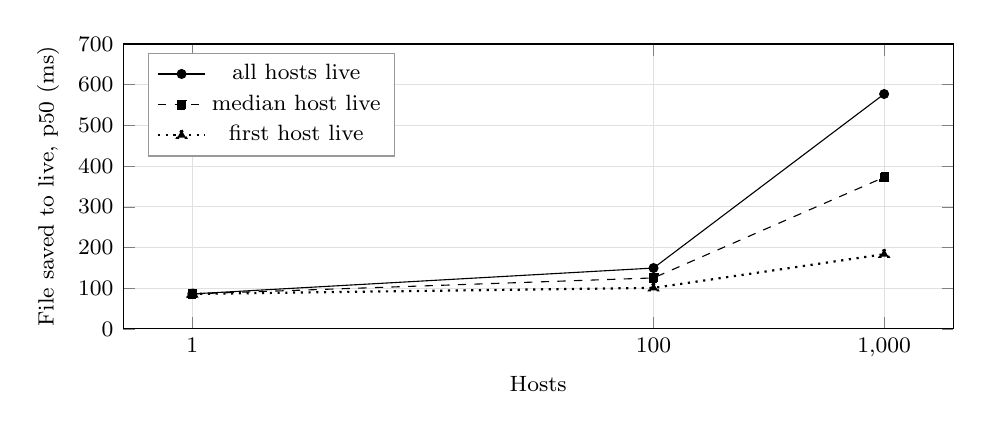
\begin{tikzpicture}
\begin{axis}[width=\columnwidth,height=5.2cm,
  xmode=log,log basis x=10,xtick={1,100,1000},xticklabels={1,100,{1,000}},
  xlabel={Hosts},ylabel={File saved to live, p50 (ms)},
  ymin=0,ymax=700,ytick={0,100,...,700},
  legend style={at={(0.03,0.97)},anchor=north west,font=\footnotesize,draw=black!40},
  tick label style={font=\footnotesize},label style={font=\footnotesize},
  grid=major,grid style={black!12}]
\addplot[black,mark=*,mark size=1.6pt] coordinates {(1,86.0) (100,149.6) (1000,577.2)};
\addlegendentry{all hosts live}
\addplot[black,dashed,mark=square*,mark size=1.6pt] coordinates {(1,86.0) (100,125.3) (1000,372.6)};
\addlegendentry{median host live}
\addplot[black,dotted,thick,mark=triangle*,mark size=1.8pt] coordinates {(1,86.0) (100,100.8) (1000,183.6)};
\addlegendentry{first host live}
\end{axis}
\end{tikzpicture}
\caption{Time from saving a layer file to hosts running it, over real WebSockets on one 4-core
machine (30, 20 and 10 trials). About 80\ms of every point is the publisher's fixed file-watch
debounce. No host rejected an update; state was kept on every host.}
\label{fig:fleet}
\end{figure}

One host is live 86\ms after the save (p95 88\ms), of which 80\ms is the publisher's fixed
file-watch debounce. All of 100 hosts are live after 150\ms (p95 164\ms) and all of 1{,}000 after
577\ms (p95 659\ms). The simulation is pessimistic in one way and optimistic in two. All hosts
verify and swap on the same four cores, so at 1{,}000 hosts per-host apply time grows from 3\ms
to about 230\ms through queueing; real devices would verify in parallel. Against that, the network
is the loopback interface, and hosts in one process share a compiled-module cache. The simulated
hosts also run layers inline rather than in workers, because hundreds of worker threads in one
process stall, so these figures exclude worker cost.

\subsection{Refusal and rollback}

Over 200 trials on one host: a version that crashes on a user action after going live is caught,
its writes discarded, the slot reverted and the UI re-rendered in 2.32\ms (p50; p95 3.30\ms), and
the host ended on the previous good version with state unchanged on every trial. A version that
fails its pre-flight check is refused before it is ever live in 7.0\ms (p50; p95 31\ms; this
includes signing the bad manifest and loading it into a fresh worker). A normal event on the good
version took 0.88\ms.

Re-running this benchmark for the paper exposed that it had gone stale. It used a schema-2 layer
as the good version and a schema-1 layer as the crashing one. After the security fix that forbids
reverting across schemas, the host correctly declined that revert, and the benchmark's own
check (``reverted to the good version on every trial'') reported \emph{false}. We changed the
benchmark to use a same-schema base, which is the case it was meant to measure, and report those
numbers. The documentation's earlier figure of 0.17\ms predates worker isolation.

\subsection{Rebuild-and-restart baseline}
\label{sec:baseline}

The same small application, written as a plain Node.js HTTP server holding its data in memory,
was redeployed on the same machine (Table~\ref{tab:baseline}).

\begin{table}[t]
\centering\footnotesize
\begin{tabular}{@{}lrr@{}}
\toprule
Flow & p50 (ms) & p95 (ms) \\
\midrule
Bare process restart until healthy & 41 & 52 \\
Docker: build (warm cache) & 255 & 284 \\
Docker: remove old container & 196 & 209 \\
Docker: start until healthy & 230 & 254 \\
\textbf{Docker total} & \textbf{681} & 726 \\
\midrule
LLP full swap (warm) & 2.3 & 3.1 \\
LLP file saved to live, one host & 86 & 88 \\
\bottomrule
\end{tabular}
\caption{Conventional redeploy versus LLP on one machine (20 restart and 10 Docker trials).
In-memory state was lost on every baseline trial and kept on every LLP trial.}
\label{tab:baseline}
\end{table}

The honest reading is that on one machine, for a trivial application, the conventional path is
\emph{not slow}: a restart takes 41\ms and a full container rebuild and replace 0.68\s. This
baseline is also a best case for it (no dependencies, no tests, no registry, one machine). LLP's
measured advantages here are qualitative: in-memory state survives, there is no window in which
the application is unreachable (the Docker flow has about 0.43\s between removing the old
container and the new one being healthy), and a bad version is refused or reverted automatically.
The large time gap between LLP and common practice lies in stages a local benchmark cannot
reproduce (hosted CI, registries, fleet rollout); for those we rely on the cited industry figures
and on the end-to-end run below.

\subsection{End-to-end: one change, two ways}
\label{sec:race}

The repository's demonstration races the same two changes through both paths at once. The
conventional side is a plain JavaScript application with API and browser end-to-end tests; a
change is committed, pushed, tested by GitHub Actions, and the server restarted. The LLP side is
the real AI publishing loop streaming to a real host in Chromium. The model's code was written in
advance and approvals are instant on both sides, so neither clock includes thinking or review
time. Table~\ref{tab:race} gives the recorded run (hosted CI) and our re-run with the same tests
executed locally.

\begin{table}[t]
\centering\footnotesize
\begin{tabular}{@{}lrr@{}}
\toprule
 & Hosted CI & Local CI \\
 & (recorded) & (re-run) \\
\midrule
\multicolumn{3}{@{}l}{\emph{Change 1: a correct change, request to live}} \\
LLP & 1.10\s & 1.26\s \\
\quad compile/check/swap (ms) & 690/234/37 & 821/215/27 \\
Conventional & 36.6\s & 3.16\s \\
Draft kept, LLP / conv. & yes / no & yes / no \\
\midrule
\multicolumn{3}{@{}l}{\emph{Change 2: an off-by-one that traps on Delete}} \\
LLP: bug reaches a device & never & never \\
LLP: corrected version live & 2.12\s & 2.76\s \\
Conv.: bug live after & 42.1\s & 5.5\s \\
Conv.: broken for users & 35.0\s & 3.7\s \\
\bottomrule
\end{tabular}
\caption{The same changes shipped both ways. Hosted CI: GitHub Actions, recorded 17 Nov 2026
(\code{docs/demo-run.json}). Local CI: the same tests in a fresh clone on the evaluation machine.}
\label{tab:race}
\end{table}

Two caveats matter. First, of the 36.6\s on hosted CI, 22\s is one workflow step that installs
the test browser without a cache. With a warm local runner the conventional path takes 3.2\s, so
the gap to LLP is about $2.5\times$, not $33\times$. The widely quoted ``1.1\s against 37\s''
describes an uncached hosted pipeline for a tiny application; a tuned pipeline would be faster and
a realistic one, with a larger test suite, slower. Second, the more robust result is not speed. In
both configurations the conventional tests passed the planted bug, which then reached users and
stayed until a revert went through the same pipeline, whereas the LLP shadow check trapped it
before any host received it and the corrected layer went live on the second attempt. In both
configurations the conventional reload discarded the user's typed draft and LLP kept it, because
the input is bound to host-owned state. The bug was planted to be the kind a click-through finds;
\S\ref{sec:security} discusses the kinds it would not.

\subsection{Server hosts}

Table~\ref{tab:server} shows a server tenant holding a shared task list of increasing size. Call
latency is flat in store size because each call carries only the keys changed since the worker's
last call; the repository records that an earlier design, which sent the whole state, cost
157\ms per event at 100{,}000 keys.
Migrating every record during a swap grows linearly and stays inside the server's limits at one
million keys. A client that mirrors the entire shared store runs out of worker memory at one
million keys; clients must subscribe to narrower prefixes. A change to a server-only slot reached
40 connected clients in 16--26\ms; a change that also swaps a client slot took 287\ms (p50). One
tenant served about 5{,}600 simple calls per second, serialised: a tenant runs one call at a
time, and a long computation delays that tenant's other calls.

\begin{table}[t]
\centering\footnotesize
\begin{tabular}{@{}lrrr@{}}
\toprule
Shared keys & 3{,}002 & 300{,}002 & 1{,}000{,}001 \\
\midrule
Call p50 (ms) & 0.14 & 0.13 & 0.08 \\
Call p99 (ms) & 0.60 & 0.47 & 49 \\
First call (ms) & 3 & 271 & 966 \\
Swap + migrate all (ms) & 39 & 745 & 2{,}793 \\
Client connect, mirror all (ms) & 85 & 1{,}544 & fails \\
Client connect, one prefix (ms) & 50 & 159 & 368 \\
\bottomrule
\end{tabular}
\caption{Server host versus shared-store size (one tenant, 50 calls per size).}
\label{tab:server}
\end{table}

The fleet controller keeps running counts per channel rather than rescanning hosts on each report;
one round of reports costs 16\ms for 2{,}000 hosts and 37\ms for 8{,}000 ($2.2\times$ for
$4\times$ the hosts). Before that fix, found by the security review, cost grew quadratically and a
10{,}000-host run did not finish in eight minutes.

\section{Failure Replays}
\label{sec:cases}

To test the protocol against failures it was not designed around, we reproduced the
\emph{mechanism} of four public incidents and one everyday pattern as small layers, and delivered
each faulty layer two ways: as the incident delivered it, and through LLP with staged rollout,
health gates, call budgets and per-host revert. Table~\ref{tab:cases} gives the results of our
re-run. Fault counts (hosts, orders, failed requests) were identical to the repository's recorded
run; times and throughput differed by up to 35\%.

\begin{table*}[t]
\centering\footnotesize
\begin{tabularx}{\textwidth}{@{}p{2.55cm}p{3.5cm}XX@{}}
\toprule
Incident & Mechanism modelled & As it happened (simulated) & Through LLP (simulated) \\
\midrule
CrowdStrike, 2024~\cite{crowdstrike2024rca} &
Update reads a 21st field from a 20-field input; out-of-bounds read traps &
1{,}000 of 1{,}000 hosts crash and crash again on reboot &
Rollout halts at its 1\% step. 10 hosts ran it, 0 went down, 10 events dropped; fleet rolled back
1.17\s after publish \\
Knight Capital, 2012~\cite{sec2013knight} &
New code reaches 7 of 8 servers; a reused flag triggers retired code on the 8th &
3{,}676 child orders for 212 parent orders; rolling the 7 good servers back raises it to 9{,}974 &
Convergence report names the 8th server at once. Flag gated on a \emph{complete} fleet: 212
orders, 0 unintended. Gated on \emph{converged}, or ungated: 243 orders (31 unintended) \\
Cloudflare, 2019~\cite{cloudflare2019} &
Backtracking pattern takes $\sim$3\s per request body &
Throughput falls from 98{,}387 to 10 requests per 2\s window over 20 edges &
Staged: 1 edge ran the rule, 1 request failed (99.998\%). Pushed to 100\% at once: 20 failed
requests (99.955\%); each edge reverted after one 100\ms kill \\
Fastly, 2021~\cite{fastly2021} &
Latent divide-by-zero shipped weeks earlier, triggered by a valid customer setting &
20 of 20 edges down; 0\% availability for every customer &
The buggy release \emph{passed} its staged rollout. On trigger: 0 edges down, 20 of 6{,}000
requests failed (99.667\%), 100\% for other customers \\
Hotfix behind a release (pattern) &
One-line pricing bug in 1{,}000 live sessions &
Not simulated &
Fix on all 1{,}000 running clients 1.83\s after publish via a 1/10/50/100\% rollout; 0 sessions lost \\
\bottomrule
\end{tabularx}
\caption{Failure mechanisms replayed in simulation (\code{npm run case-studies}, 17 checks, all
passing). Fleets run in one process with 1--10\ms of simulated message delay. These are replays of
mechanisms, not reconstructions of the affected systems, and not claims that LLP would have
prevented the incidents.}
\label{tab:cases}
\end{table*}

\paragraph{What the replays show.} For faults that trap or hang, containment came from two
independent mechanisms. Staged rollout limited how many hosts met the fault. The transactional
event rule and the call budget meant that hosts which did meet it lost one event or one request
and kept serving on the previous version. The second mechanism mattered on its own: with staging
disabled in the Cloudflare replay, availability was still 99.955\%, and in the Fastly replay,
where staging was irrelevant, no edge went down.

\paragraph{Where LLP did not help.} We consider these as important as the results above.
\begin{itemize}
\item \emph{Wrong but running.} Knight's root cause was semantic: a reused flag and dead code.
Nothing trapped, so no budget, shadow check or revert saw anything. LLP limited damage only
through convergence tracking and a gate that an operator must choose to use. Moreover ``one swap
rolls everything back'' is exactly the action that made Knight's morning worse.
\item \emph{A defect in LLP itself.} The replay showed that gating on \code{converged}, which
ignored offline hosts by design, was no better than not gating at all. We added \code{complete}.
As first written, the protocol's gate would not have prevented the failure.
\item \emph{Data is not code.} In the Fastly replay the trigger was a configuration value, which
reaches every host at once. LLP stages and shadow-checks code, not data. There is no shadow check
for a configuration change.
\item \emph{The pre-flight run is shallow.} The CrowdStrike layer failed only on an event, so the
shadow check passed it and the first live event caught it. For a security product one dropped
event can be one missed detection.
\item \emph{Reach.} The real CrowdStrike component runs in the operating-system kernel, where a
user-space WebAssembly host cannot reach. Reverting the Cloudflare rule keeps the edge serving but
without the protection the rule was meant to add.
\item \emph{Recovery depends on a good predecessor.} The Fastly revert works only because the
previous release lacked the bug. Had every retained version contained it, each triggering request
would fail, though others would still be served.
\item \emph{Fidelity.} The legacy columns can be worse than reality (0\% in our Fastly replay
against the roughly 15\% of the network that kept working), because every simulated edge receives
the triggering traffic. Fleet sizes stop at 1{,}000 hosts. The hotfix pattern has no measured
conventional side.
\end{itemize}

\section{Security Analysis}
\label{sec:security}

\subsection{Threat model}

We consider: a network attacker who can read and alter traffic; a relay, CDN or server host that
can delay, drop or replay releases; an application user sending arbitrary input; a third-party or
machine-written layer running inside the host; a publisher (human or model) that is mistaken or
misled; a leaked release key and a leaked root key; another program on the same device; and a
party holding a copy of the disk. LLP does not defend against a compromised host runtime or
operating system, and v0 offers no defence against denial of service on the publisher or
controller beyond message size limits.

\subsection{Red-team review}

An adversarial review of the specification and reference code produced 39 findings, six of them
demonstrated by a script that runs the real code. Table~\ref{tab:redteam} lists the most serious.
Every fixed finding has a test asserting the safe behaviour (71 checks in total), and the
demonstration script now reports that none of the six still holds.

\begin{table}[t]
\centering\footnotesize
\begin{tabularx}{\columnwidth}{@{}lX@{}}
\toprule
ID & Finding (as found) $\rightarrow$ status \\
\midrule
RT-01 & A host with an empty key list skipped the signature check entirely. \emph{Critical.}
$\rightarrow$ Fixed: fail closed. \\
RT-02 & One huge version number froze all future updates. $\rightarrow$ Fixed: bounded versions,
key epochs. \\
RT-03 & The fleet controller trusted a host's claimed name. $\rightarrow$ Fixed: device keys and
a challenge. \\
RT-04 & Layers on one host shared all state. $\rightarrow$ Fixed, opt-in: declared keys. \\
ST-01 & A revert after a migration ran old code on new data. $\rightarrow$ Fixed. \\
ST-02 & Server data was memory-only. \emph{Critical for backends.} $\rightarrow$ Fixed for one
node; no replication. \\
CO-01 & One user's failing call rolled the server back for everyone. $\rightarrow$ Fixed:
revert only after failures from several users. \\
AI-01 & Text from any reachable host was fed to the model unfiltered. $\rightarrow$ Fixed:
loopback by default; feedback quoted and capped. \\
AI-03 & Every layer got every capability. $\rightarrow$ Fixed, opt-in: declared capabilities. \\
SEC-01 & A relay could hold a device on an old release. $\rightarrow$ Fixed, opt-in, fleet hosts
only. \\
\bottomrule
\end{tabularx}
\caption{Selected red-team findings. Full list and status: \code{docs/RED-TEAM.md}.}
\label{tab:redteam}
\end{table}

Of the 39 findings, 29 are marked fixed. That figure overstates the position unless qualified.
Seven of the 29 are fixed only partly (size limits, read rules on shared data, key custody, state
quotas, prompt hygiene, per-person export and erasure, and encryption at rest). Three are opt-in
manifest or host features (state isolation, declared capabilities, freshness); a v0 manifest does
not get the first two unless it declares \code{"llp": 1}. Durable server state, effect records
and encryption at rest apply only when the operator configures a data directory or a data key. Several fixes changed behaviour in ways an
embedder must know, notably that a host created without keys now refuses every manifest.

\subsection{Open findings}

Ten findings remain open:
\begin{itemize}
\item \textbf{AI-02.} The approval screen includes a summary written by the model. A
tool-computed summary (keys written, capabilities, schema change) is only partly built.
\item \textbf{AI-04.} The shadow check covers what it happens to try. Faults that need many
events, a date or unusual input pass. Machine-written releases should go through a staged rollout
by default and applications should be able to ship invariants; neither is built.
\item \textbf{CO-03.} Time limits are wall-clock, not CPU time.
\item \textbf{PERF-01.} A tenant runs one call at a time, and one user can fill its queue.
\item \textbf{OB-02.} Fleet reports are authenticated but their content is the host's own word;
they are suitable for gating rollouts, not as proof of what code a host runs.
\item \textbf{OB-03.} No standard traces or metrics; logs from a killed call are lost.
\item \textbf{PR-04.} No signed, append-only public log of releases in the style of a
transparency log~\cite{newman2022sigstore}.
\item \textbf{GOV-02.} Addressed for the client role by the Go host and the vectors; the server
role still has a single implementation.
\item \textbf{GOV-03.} The ABI is bespoke rather than defined in the WebAssembly Component
Model~\cite{componentmodel}.
\item \textbf{GOV-04.} The code is now public under Apache-2.0, but there is no change process or
neutral governance.
\end{itemize}

Beyond these: release manifests carry one signature (thresholds exist only for the root role);
freshness notes are signed with the release key rather than a separate timestamp key; hosts
outside a fleet have no freshness check; keys are files, with no hardware or keystore API; and
trust-on-first-use enrollment lets whoever first claims a host id own it. The WebAssembly sandbox
protects the host from a layer; it does not make a layer's own memory safe~\cite{lehmann2020wasm}.
The keyring rotation logic has tests but has not been model-checked.

\section{Related Work}
\label{sec:related}

\paragraph{Dynamic software updating.} A long line of research updates running programs without
stopping them: for C~\cite{hicks2005dsu,neamtiu2006ginseng,hayden2012kitsune}, for managed
runtimes~\cite{subramanian2009jvolve}, for operating-system kernels~\cite{arnold2009ksplice} and
for whole operating systems~\cite{giuffrida2013proteos}. These systems patch a program in place
and must find safe update points and transform live heap state. LLP sidesteps the hardest part by
construction: layers hold no state between calls, so every call boundary is a safe point and the
only state transformation is an explicit, versioned migration over a key/value store. The price is
a constrained programming model. Erlang/OTP~\cite{armstrong2003} is the closest in spirit, with
state held outside replaceable code and a \code{code\_change} hook; it is one language, server
side, and has no pre-commit rehearsal or signed delivery.

\paragraph{Secure update frameworks.} TUF~\cite{samuel2010tuf} defines roles, thresholds and
defences against rollback and freeze attacks; Uptane~\cite{kuppusamy2016uptane} adapts it to
vehicles; Sigstore~\cite{newman2022sigstore} provides signing and transparency logs. LLP adopts
TUF's root and release roles and its chained rotation, and currently lacks its timestamp and
snapshot roles and Sigstore-style transparency. LLP is not an alternative to these; a mature
version should use them.

\paragraph{Safe deployment.} Staged rollout with automated health decisions is established
practice at scale~\cite{li2020gandalf}, and configuration is known to be as dangerous as
code~\cite{tang2015config}. LLP's rollout gates are a small instance of the former. Its lack of
any staging for data is the gap the latter warns about.

\paragraph{Over-the-air application updates.} Expo's EAS Update~\cite{expoupdates},
Shorebird~\cite{shorebird2025} and Capgo~\cite{capgo} push new code to installed mobile
applications, with channels, rollouts and rollback, at large scale. Each is tied to one framework,
and updates take effect at the next launch rather than as an in-place swap with state kept. We
did not find pre-commit verification against live state in their documentation; our survey read
public documentation only and may have missed features.

\paragraph{Declarative agent-to-UI protocols.} A2UI~\cite{a2ui} lets an agent stream interface
descriptions rendered with an application's native components, and is explicitly declarative, not
executable. MCP Apps~\cite{mcpapps} ships HTML and JavaScript rendered in a sandboxed frame inside
AI chat hosts. Both address ``an agent changes what the user sees''. Neither defines versioned
executable logic, state migration, or swap and rollback semantics. The declarative approach is
safer by construction, and for many uses sufficient.

\paragraph{WebAssembly platforms.} Cloudflare's Dynamic Workers~\cite{dynamicworkers} start
isolates at run time from generated code, aimed at AI-written programs. Fermyon Spin and
wasmCloud~\cite{wasmcloud} run WebAssembly components on servers; wasmCloud can replace a
component without dropping invocations. These are server-side and, in what we read, do not carry
state across a swap or rehearse on live state. Extism~\cite{extism} is a cross-language plug-in
framework that could serve as a building block. Content-addressed code is central to
Unison~\cite{unison}.

\paragraph{Development-time hot reload.} Hot module replacement and its descendants swap code in a
running program during development. They are unsigned, unverified, and intended for one
developer's machine; LLP can be read as an attempt to give that experience the guarantees
production needs.

\paragraph{What is new.} Each mechanism in LLP has prior art. To our knowledge the combination
does not: one signed, monotonic stream for client and server hosts; host-owned state with
versioned migration; rehearsal on a shadow of the real state before an atomic commit; per-call
transactions with automatic revert; and delivery designed for a machine publisher. We searched
public sources and cannot rule out systems we did not find.

\section{Limitations and Future Work}
\label{sec:limits}

\paragraph{Evidence.} There is no production deployment. Fleets and outages are simulated on one
machine with loopback networking. The layers are a few kilobytes; swap cost for large modules and
for migrations touching much state on a client is unmeasured. Both implementations were produced
within one project over a few days, with heavy use of an AI coding assistant, so ``independent''
means written from the specification without porting code, not written by a separate team.

\paragraph{What the checks miss.} LLP detects layers that fail to load, trap, hang or exhaust
memory. It does not detect a layer that runs and computes the wrong thing. This is the most
important limitation for machine-written code. The pre-flight run exercises one render. Staged
rollout only helps if a failure surfaces as a trap, a revert or a metric someone gates on.

\paragraph{Expressiveness.} The UI vocabulary has eleven element kinds and no canvas, frame loop,
audio or accessibility metadata, so v0 suits forms and lists, not rich or real-time interfaces.
Layers on one host cannot call each other. There is no host for constrained devices.

\paragraph{Server side.} One writer per tenant, one process per tenant, no replication or
failover, and about 9\,MB per busy tenant worker. Clients behind a server host report to that
server, not to the fleet controller, so convergence counts see the server and not the devices
behind it.

\paragraph{Platform policy.} Some application distribution platforms restrict downloading
executable code. Whether sandboxed, capability-mediated WebAssembly falls inside their exemptions
for interpreted code is untested. We leave this out of scope and note that desktop, web and server
environments impose no such gate.

\paragraph{Future work.} In rough priority: staged rollout and shadow checks for data and
configuration; application-supplied invariants evaluated after each event; CPU-time limits; a
second implementation of the server role with vectors; a WIT definition of the ABI; a transparency
log; threshold signatures and hardware custody for release keys; a richer rendering surface; and
measurement on real devices over real networks.

\section{Conclusion}

LLP asks whether the checks a delivery pipeline performs can be performed instead by the program
that receives the change, at the moment it arrives, on the state it will actually run against.
For a constrained class of applications the answer in our prototype is yes: a signed layer is
verified, rehearsed and swapped in a few milliseconds with state intact, a crashing layer is
reverted in a few more, and two implementations agree on 161 checks. The measurements also correct
an easy overstatement. On one machine a restart is fast; what LLP changes is that state survives,
nothing is unreachable, and failure is contained per host and per call. The failure replays and
the security review mark the boundary clearly: crashes and hangs are contained, wrong answers and
bad data are not. We publish the specification, both hosts, the vectors, the benchmarks and the
open findings so that the claims here can be re-run and the boundary pushed.

\section*{Artifact Availability}

Everything is at \repo{} under Apache-2.0. \code{npm test} runs the 428 checks;
\code{npm run test:go} the Go host; \code{npm run bench}, \code{npm run bench:hosts} and
\code{npm run case-studies} regenerate the measurements; \code{npm run redteam} re-checks the
demonstrated findings. The raw output behind every number in this paper is in
\code{paper/results/}.

\section*{Acknowledgements and AI Disclosure}

The specification, both implementations, the tests and this manuscript were written with
substantial assistance from Anthropic's Claude models, directed and reviewed by the author. Every
quantitative claim was produced by running the scripts named above. The author is responsible for
the content.

\bibliographystyle{unsrt}
\bibliography{refs}

\end{document}
